% !TEX root = ../thesis.tex

\chapter{Experimental Setup}
\label{chap:exp}

\section{Introduction}

% Accelerators vs. cosmic rays
Accelerators have been at the heart of particle and nuclear physics since they first came online in the mid-20th century.
Initial experiments that established the existence of familiar particles such as muons and pions utilized cosmic rays, and cosmic rays are still used today for various projects such as the IceCube Neutrino Observatory~\cite{Abbasi_2009}.
However, accelerator facilities offer numerous advantages over using cosmic rays.
One is that the energies of the beams may be controlled by experimenters, which allows for studying the energy dependence of interactions.
Another is that the projectile type in the beam may be chosen in order to select for certain interactions.
Finally, the interactions take place at a specified location where detectors may be located.

% Fixed-target accelerators
The center-of-mass energy \ECM\footnotemark{} is a defining feature of an accelerator, as it is a measure of the energy available to produce particles in collision events~\cite{martin2008particle}.
\footnotetext{Sometimes instead written in terms of the Mandelstam variable $s$ as $\sqrt{s}=\ECM$~\cite{Perelstein_2011}.}
There are two types of accelerators to consider: fixed-target and colliders. % Check terms
A key distinction between them is how they differ their center-of-mass energies based on the parameters of the accelerator.
Fixed-target accelerators involve a single beam that is directed to a stationary target in the lab frame, with a center-of-mass energy given by
\begin{equation}
  \ECM=\sqrt{m_b^2c^4+m_t^2c^4+2m_tc^2E_L},
\end{equation}
where $m_b$ is the mass of the particles in the beam, $m_t$ is the mass of the particles in the stationary target, and $E_L$ is the energy of the beam as measured in the lab frame.
While the beam energy can be calibrated, this form of \ECM goes as $\sqrt{E_L}$ for high beam energies.

% Colliders
On the other hand, colliders involve two beams of particles that are directed to cross into each other and collide at a fixed position where the detectors are located.
In this case, given two beams with energies $E_{L,1}$ and $E_{L,2}$ as measured in the lab frame, the center-of-mass energy is simply
\begin{equation}
  \ECM=E_{L,1}+E_{L,2},
\end{equation}
and if $E_{L,1}=E_{L,2}=E_L$, this reduces to $\ECM=2E_L$.
Thus, colliders have the advantage that they depend linearly on beam energy and therefore have higher gains in \ECM compared to fixed-target accelerators.

% Luminosity
Another key parameter of an accelerator is the luminosity $\mathcal{L}$.
Given a cross section $\sigma$ for a process, and a rate at which events occur $R$, the luminosity is the constant of proportionality such that
\begin{equation}\label{eq:evtRate}
  R=\mathcal{L}\sigma,
\end{equation}
where $\mathcal{L}$ has units of cm$^{-2}$s$^{-1}$. % Check how to stylize units
In some cases it is useful to instead consider the time integral of the luminosity $\mathcal{L}_\mathrm{int}$, which is given by
\begin{equation}
  \mathcal{L}_\mathrm{int}=\int\mathcal{L}\dd{t}.
\end{equation}
This can then be used with equation~\ref{eq:evtRate} to obtain the number of collision events $N_\mathrm{event}$ for a process:
\begin{equation}
  N_\mathrm{event}=\mathcal{L}_\mathrm{int}\sigma.
\end{equation}
Thus, by increasing the luminosity (and hence the integrated luminosity), we may increase the number of collision events of interest for a given process.
The luminosity may also be expressed in terms of parameters relevant to the beam, as it is essentially an instantaneous measure of particle flux. % Check wording
For example, given the number of particles per bunch for two Gaussian beams $N_1$ and $N_2$, revolution frequency $f$, and number of bunches $N_b$, the luminosity is
\begin{equation}
  \mathcal{L}=f\frac{N_1N_2N_b}{4\pi\sigma_x\sigma_y},
\end{equation}
where $\sigma_x$ and $\sigma_y$ are the standard deviations in the $x$ and $y$ directions for the beam distributions~\cite{Herr:941318}.

% Discoveries at colliders
The search for new physics has driven advances in accelerator center-of-mass energies and luminosities that allow for discovering exotic collision events.
Figure~\ref{fig:ECMplot} shows the constituent center-of-mass energies for various accelerator facilities as a function of the year in which they came online~\cite{Panofsky}.
These advances have resulted in the discovery of massive particles that the first accelerators in the 1960's were not capable of producing, such as the $W$ and $Z$ bosons, or the top quark. % Check wording
Even following the success of the Higgs boson discovery in 2012 and the ongoing search for new particles at the LHC, there are still upgrades being installed on the LHC to increase its luminosity, and there are proposals for new accelerator facilities with higher center-of-mass energies~\cite{Bicer_2014}.

\begin{figure}[htbp]
  \centering
  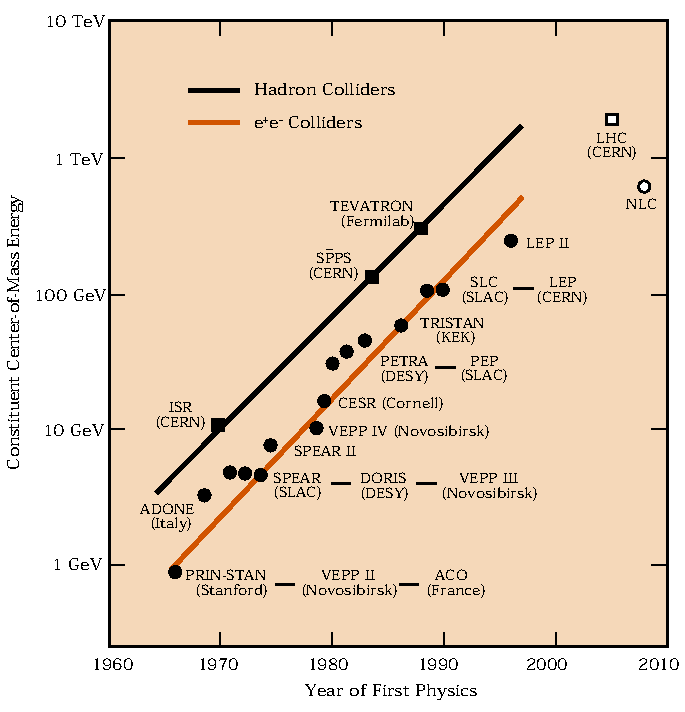
\includegraphics[width=0.5\textwidth]{fig/experiment/ecm_livingston.pdf}
  \caption{
    Plot of the constituent center-of-mass energies for hadronic and $e^+e^-$ colliders since 1960.
    The discovery of massive particles such as the $W$ and $Z$ bosons or the top quark was made possible thanks to advances in accelerator technology that allowed for higher center-of-mass energies and luminosities.
  }
  \label{fig:ECMplot}
\end{figure}

% Chapter overview
This chapter explores the main features of the Large Hadron Collider facility at CERN in section~\ref{sec:LHC}, where collision events used in the search were obtained.
A complete documentation of the LHC machine can be found in reference~\cite{Evans:1129806}.
We then turn our attention to the Compact Muon Solenoid detector in section~\ref{sec:CMS} and briefly go over the main components of the device, which was used to record the collision events at the LHC.
This overview is based off of documents concerning CMS in references~\cite{Chatrchyan:1129810,taylor_2011}.

\section{The Large Hadron Collider}
\label{sec:LHC}

% The Large Hadron Collider
The Large Hadron Collider is a circular collider accelerator facility with two superconducting rings that accelerate protons to relativistic speeds, and it is located just outside of Geneva on the French-Swiss border.
It is the largest and most powerful collider in the world, with plans to extend its service life into the 2030's and 2040's.
It has a circumference of 26.7 km and was built into an existing tunnel that was used for the Large Electron-Positron (LEP) collider, which was used from 1989 to 2000.
Various detectors used to study collision events are placed along the beamline, such as ALICE, ATLAS, CMS, and LHCb.
Figure~\ref{fig:CERN} shows the complete CERN accelerator complex with all of its components~\cite{Mobs:2636343}.
The ATLAS and CMS facilities are general-purpose detectors for studying the Higgs and searching new physics arising from proton-proton collisions, while ALICE is optimized for studying heavy-ion collisions with stripped lead ions ($^{208}$Pb$^{82+}$) to investigate properties of quark-gluon plasma, and LHCb is designed to study the physics of bottom quarks and $CP$ violation in $b$-hadron interactions.

\begin{figure}[htbp]
  \centering
  \includegraphics[width=0.85\textwidth]{fig/experiment/CCC-v2018-print-v2.pdf}
  \caption{
    Layout of the CERN accelerator complex.
    The LHC is one of several accelerators present at the facility, with multiple detectors along the beamline such as ATLAS, CMS, ALICE, and LHCb.
    ATLAS and CMS are both general-purpose detectors for studying properties of the Higgs and searching for new physics.
    ALICE is designed to study heavy-ion collisions with lead ions to investigate quark-gluon plasma.
    LHCb is meant to study the physics of bottom quarks and $CP$ violation in $b$-hadron interactions.
    The LHC is injected with protons and lead ions through a multi-stage process.
    Protons starting at the Linac2 facility, which are then fed through the Proton Synchrotron Booster (PSB), then to the Proton Synchrotron (PS), and then to the Super Proton Synchrotron (SPS) before finally being injected into the LHC itself.
    The lead ions undergo a similar process, starting at Linac3 and then being transferred to the Low Energy Ion Ring (LEIR), then going through the PS and SPS before being injected into the LHC.
  }
  \label{fig:CERN}
\end{figure}

% Beam injection for LHC
The LHC beam is fed through a multi-stage process in which protons are stripped off of hydrogen atoms and are first accelerated through a series of preaccelerators before being injected into the LHC beam.
Protons start at the Linac2 facility, where they are initially accelerated to $50\unit{MeV}$ before being transferred to the Proton Synchrotron Booster (PSB) and reach $1.4\unit{GeV}$.
They are then sent to the Proton Synchrotron (PS) where they reach energies of $25\unit{GeV}$, and then they are accelerated further to $450\unit{GeV}$ at the Super Proton Synchrotron (SPS).
The protons then reach the LHC where they are accelerated to $6.5\unit{TeV}$ each.
The process is similar for lead ions, where they instead start at Linac3 with $4.2\unit{MeV/n}$, then move through the Low Energy Ion Ring (LEIR) before being transferred to the PS, then the SPS, then injected into the LHC.

% Center-of-mass energy and luminosity
While the LHC was built with the intent of achieving center-of-mass energies of $\sqrt{s}=14\unit{TeV}$ in proton-proton collisions, the data collected for this work was over a period in which the center-of-mass energy was $\sqrt{s}=13\unit{TeV}$.
It also has a specific expression for the luminosity $\mathcal{L}$ given by
\begin{equation}
  \mathcal{L}=\frac{N_b^2n_bf_\mathrm{rev}\gamma_r}{4\pi\epsilon_n\beta^*}F,
\end{equation}
where $N_b$ is the number of particles per bunch, $n_b$ is the number of bunches per beam, $f_\mathrm{rev}$ is the revolution frequency, $\gamma_r$ is the Lorentz factor, $\epsilon_n$ is the normalized transverse beam emittance, $\beta^*$ is the beta function at the collision point, and $F$ is the geometric luminosity reduction factor.
The LHC is designed to reach a luminosity of $10^{34}\unit{cm^{-2}s^{-1}}$, but surpassed this value in June 2016~\cite{LHClumi}.
Figure~\ref{fig:CMSlumi} shows the integrated luminosities as a function of time delivered to the CMS detector for the years 2015-2018~\cite{CMSlumi}.
Both ATLAS and CMS are the main high luminosity experiments, with integrated luminosities of $41.0\unit{fb^{-1}}$, $49.8\unit{fb^{-1}}$, and $67.9\unit{fb^{-1}}$ delivered to CMS over the Run 2 years of 2016, 2017, and 2018 respectively.
This corresponds to a total integrated luminosity of $158.7\unit{fb^{-1}}$ at CMS over Run 2.

% Need to check where luminosity figures used in analysis come from
%Both ATLAS and CMS are the main high luminosity experiments, with integrated luminosities of $35.9\unit{fb^{-1}}$, $41.5\unit{fb^{-1}}$, and $59.7\unit{fb^{-1}}$ recorded at CMS over the Run 2 years 2016, 2017, and 2018 respectively.
%This corresponds to a total integrated luminosity of $137.1\unit{fb^{-1}}$ at CMS over Run 2.

\begin{figure}[htbp]
  \centering
  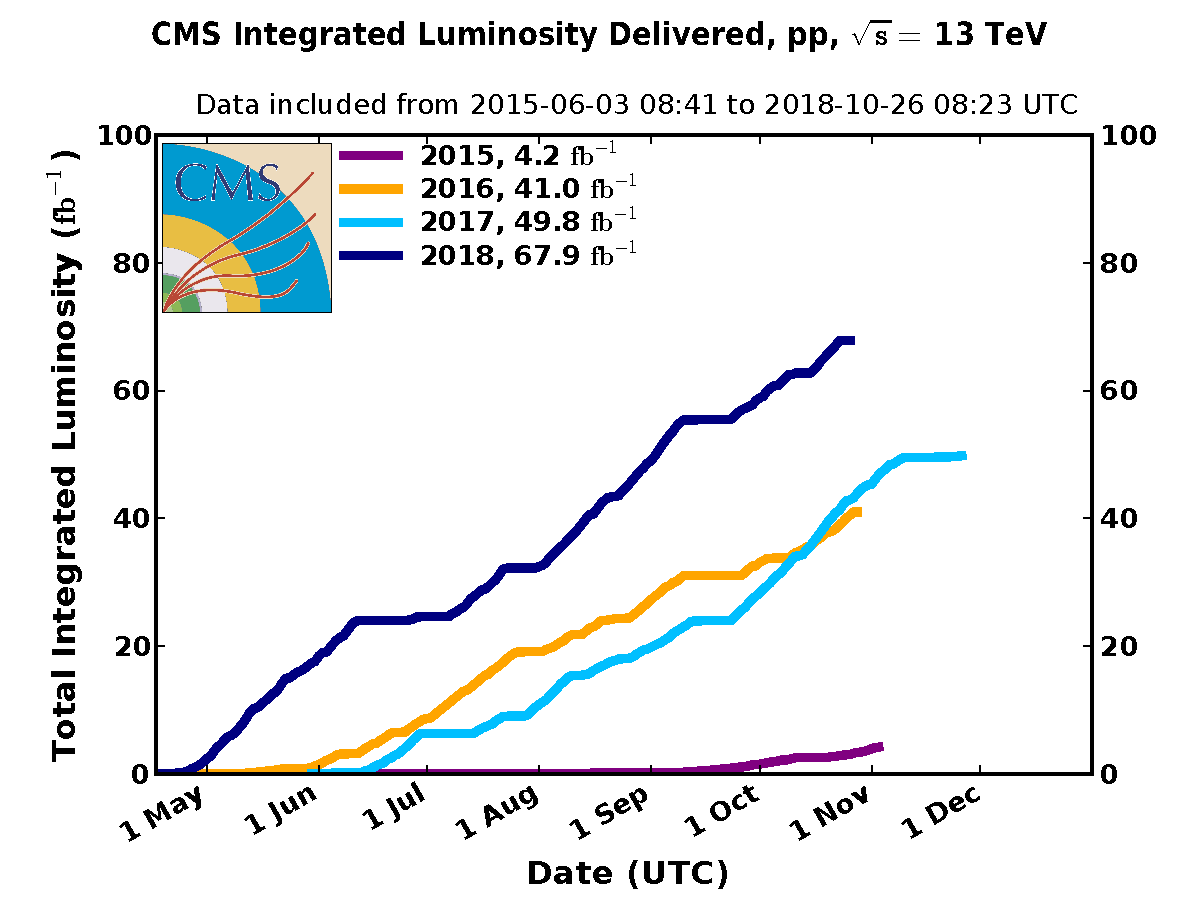
\includegraphics[width=0.65\textwidth]{fig/experiment/int_lumi_cumulative_pp_2_run2.pdf}
  \caption{
    Integrated luminosities delivered to CMS as a function of time for the years 2015-2018.
    This corresponds to a total integrated luminosity of $158.7\unit{fb^{-1}}$ delivered to CMS during the Run 2 years of 2016-2018.
  }
  \label{fig:CMSlumi}
\end{figure}

\section{The Compact Muon Solenoid}
\label{sec:CMS}

% The Compact Muon Solenoid
The Compact Muon Solenoid is one of the main general-purpose detectors at the LHC, and it along with ATLAS obtained independent results for the discovery of the Higgs boson in 2012.
The CMS detector is located 100 meters underground on the French side of the border near the village of Cessy.
It is a cylindrical apparatus with a solenoidal magnet that is coaxial with the beamline of the LHC, with a diameter of $14.6\unit{m}$ and a length of $21.6\unit{m}$, and it is surrounded by various detection systems.
The coordinate system used by CMS is defined such that $z$-axis is defined to lie along the LHC beam, with the $y$-axis pointing vertically upward and the $x$-axis pointing radially inward.
This leads to the azimuthal angle $\phi$ being measured from the $x$-axis in the $x$-$y$ plane, with the radial coordinate denoted by $r$.
The polar angle $\theta$ is defined with respect to the $z$-axis, but in practice one typically uses pseudorapidity defined by $\eta=-\ln\tan(\theta/2)$.

% Function and design overview
One of its primary functions is to accurately identify the charge and momentum of muons emerging from collision events as their trajectories are bent through the magnetic field.
Muons are ideal for reconstructing collisions due to their relatively long lifetime ($\tau_\mu=2.2\unit{\micro s}$), large mass ($m_\mu=105.7\unit{MeV/\clight^2}$), and low radiation losses when propagating through matter~\cite{peskin2019}.
This makes muons the most penetrative and easily identifiable charged particles that can be found in collision events. % Check wording
In addition to identifying muons, the CMS detector also has other components for detecting electrons, photons, and hadrons.
These detection systems are designed in order to meet the demands that come with the LHC's high luminosity, as there are more than 20 proton-proton interactions every $25\unit{ns}$, which results in around 1000 particles emerging for each bunch crossing. % Check numbers
A cutaway diagram of the detector with various components labeled may be seen in figure~\ref{fig:CMScut}~\cite{Sakuma:2665537}.

\begin{figure}[htbp]
  \centering
  \includegraphics[width=0.85\textwidth]{fig/experiment/cms_cutaway.pdf}
  \caption{
    Cutaway diagram of the CMS detector with components labeled as configured in 2018 for Run 2.
    The detector and its components are coaxial with the LHC beam and give wide geometric coverage over the interaction point where the collisions are produced.
    The silicon tracker is used to measure the initial trajectories of charged particles emerging from collisions.
    Outside of the tracker is the preshower detector that screens neutral pions and the electromagnetic calorimeter for detecting electrons and photons.
    The electromagnetic calorimeter is encased by the hadronic calorimeter, which detects hadron jets and neutrinos or exotic particles through missing transverse energy.
    Both calorimeters are surrounded by the muon detection chambers embedded within the return yoke that are used to identify muon charges and momenta.
    Finally, the Cerenkov-based forward calorimeter has both an electromagnetic and hadronic section, lying just outside of the endcaps for the muon chambers. % Check wording
  }
  \label{fig:CMScut}
\end{figure}

% Details on solenoid
One of the central components of the detector is the superconducting solenoid, a $13\unit{m}$ long and $6\unit{m}$ inner diameter magnet that provides a $4\unit{T}$ magnetic field for bending charged particles while operating at a temperature of $4.45\unit{K}$.
The field generated by the solenoid has a nominal current of $19.14\unit{kA}$, an inductance of $14.2\unit{H}$, and a stored energy of $2.6\unit{GJ}$.
The solenoid is supplemented by a $12,500\unit{t}$ flux return yoke that pulls the magnetic field lines back into the muon chambers to allow for high resolution detection of muons produced in collision events.
There are five wheels and two endcaps that comprise this return yoke, with four layers of detection chambers in both the wheels and the endcaps.

\subsection{Inner Tracking System}
\label{subsec:tracking}

% The inner tracker
The inner tracking system measures the momenta of charged particles emerging from collisions and is used to reconstruct secondary vertices for events.
One of the key aspects of the tracking system is the need to choose a design that results in minimal energy loss in charged particles passing through the detector, as this is needed to retain an accurate measurement of their trajectories. % Check wording
Additionally, in order to meet the demands that come with the severe radiation damage that occurs from the large particle flux, the need for efficient cooling, and the level of granularity necessary to measure the tracks of charged particles, the tracking system is based entirely on silicon detectors.
The tracker is $5.8\unit{m}$ long and has a diameter of $2.5\unit{m}$, surrounding the interaction point where collisions occur.
It has a pixel detector with three barrel layers that span radii from $4.4\unit{cm}$ to $10.2\unit{cm}$, as well as a silicon strip tracker with ten layers that extends to a radius of about $1.1\unit{m}$.
Both the pixel detector and silicon strip tracker have endcaps that allow for an acceptance of $|\eta|<2.5$.
% Possibly elaborate

\subsubsection{The Pixel Detector}

% The pixel detector
The pixel detector allows for precise tracking and small impact parameter resolution, which is crucial for secondary vertex reconstruction.
It covers a total area of around $1\unit{m^2}$ and is comprised of 66 million pixels.
The detector has very high efficiency in the barrel region, with losses in efficiency starting around $|\eta|>2.1$. % Possibly insert efficiency graph here
Each pixel cell occupies an area of $100\times150\unit{\micro m^2}$, which allows for high track resolution in the $r$-$\phi$ plane and in the $z$ direction.
Figure~\ref{fig:CMSpixel} shows an illustration of the pixel detector~\cite{Collaboration_2010_pixel}.
As charged particles pass through a silicon pixel, they impart energy onto the electrons in the silicon atoms, which ejects the electrons and generates a current that goes into a readout chip attached to the pixel.
Each pixel consumes about $55\unit{\micro W}$ of power, which results in $3.6\unit{kW}$ of power for the entirety of the pixel detector.
To avoid overheating from the power consumption, the pixels are mounted on cooling tubes, with 10 for the barrel and 4 for the two end disks.

\begin{figure}[htbp]
  \centering
  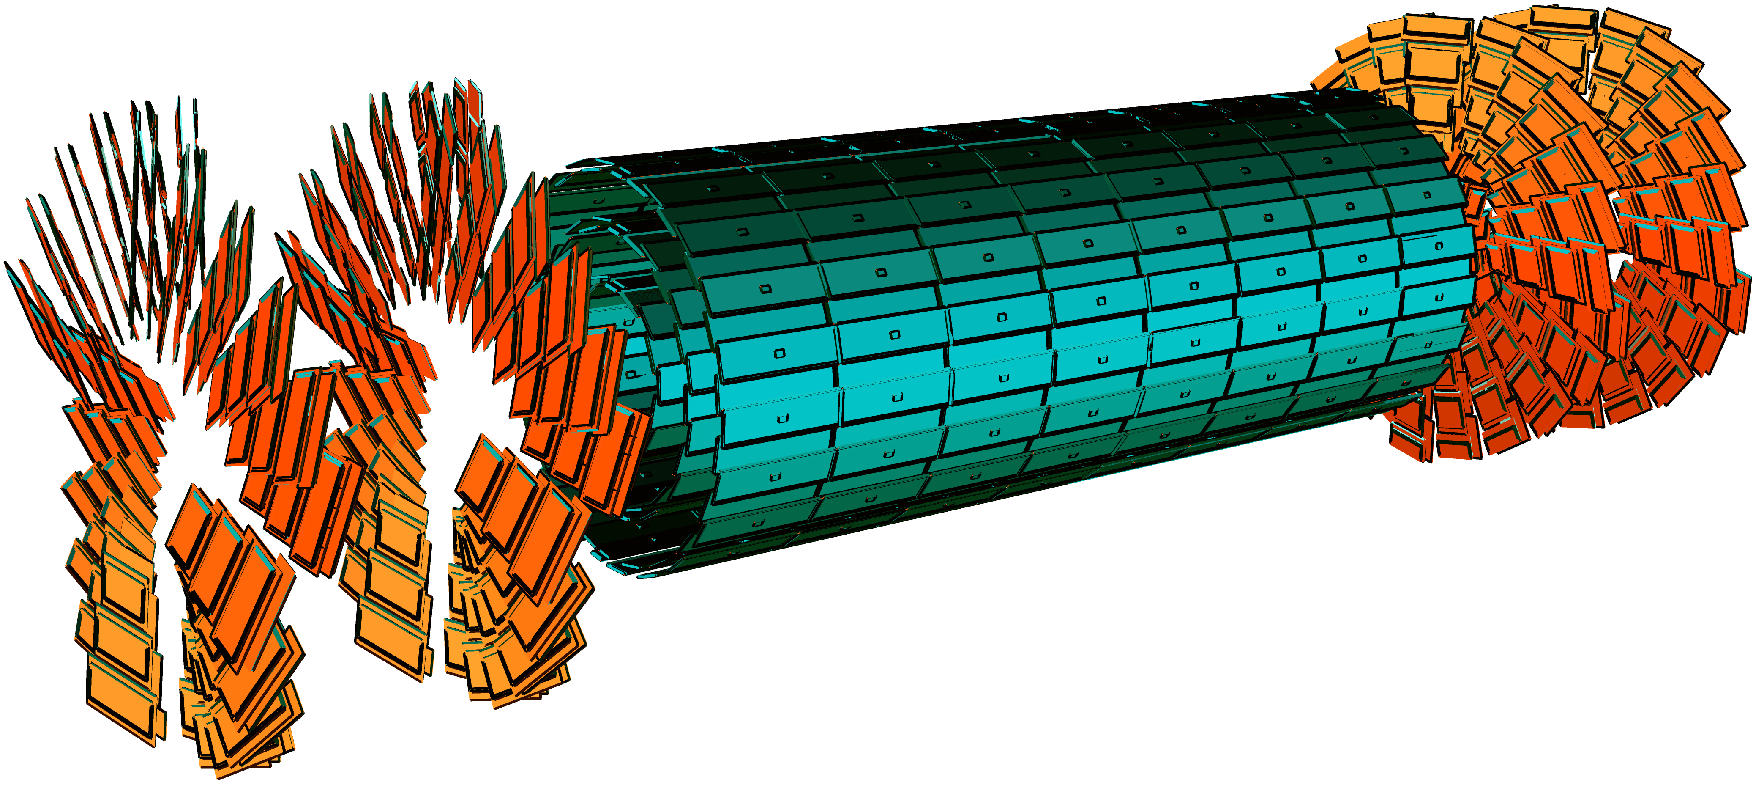
\includegraphics[width=0.85\textwidth]{fig/experiment/cms_pixelTracker.pdf}
  \caption{
    Illustration of the CMS pixel detector, with the barrel region colored in blue, and the endcap regions colored in orange.
    A current is generated as charged particles pass through the pixel cells and eject electrons, which is read by a readout chip attached to each pixel.
  }
  \label{fig:CMSpixel}
\end{figure}

\subsubsection{The Silicon Strip Tracker}

% The silicon strip tracker
Once particles pass through the three layers of the pixel detector, they then go through the silicon strip tracker.
The strip tracker has 15,148 detector modules in total, spread out among several layers, with each module containing 24,244 silicon sensors along with electronic readouts supported by a carbon fiber or graphite frame. % Check wording
These strips work in a manner similar to the pixels, with electrons getting knocked out of the material as charged particles pass through them and sending a current to be read out by a sensor.
Figure~\ref{fig:CMSsilicon} shows the layout of the strip tracker~\cite{Chatrchyan:1211825}.
The Tracker Inner Barrel (TIB) has four inner barrel layers of silicon strips placed between radii of $255.0\unit{mm}$ and $498.0\unit{mm}$, which has a length of $1.4\unit{m}$ along the LHC beamline centered at the interaction point.
The TIB is closed off by the Tracker Inner Disks (TID), with the two endcaps containing three disks each placed along the $z$ axis between $\pm800\unit{mm}$ and $\pm900\unit{mm}$ from the interaction point.
The Tracker Outer Barrel (TOB) consists of two double-sided layers of silicon strips just outside the TIB, followed by four single-sided layers, with the layers having radii between $608\unit{mm}$ and $1080\unit{mm}$.
The TOB is closed off by the Tracker EndCaps (TEC) which extend radially from $220\unit{mm}$ to $1135\unit{mm}$ and from $\pm1240\unit{mm}$ to $\pm2800\unit{mm}$ along the beamline.

\begin{figure}[htbp] % Want a higher quality figure
  \centering
  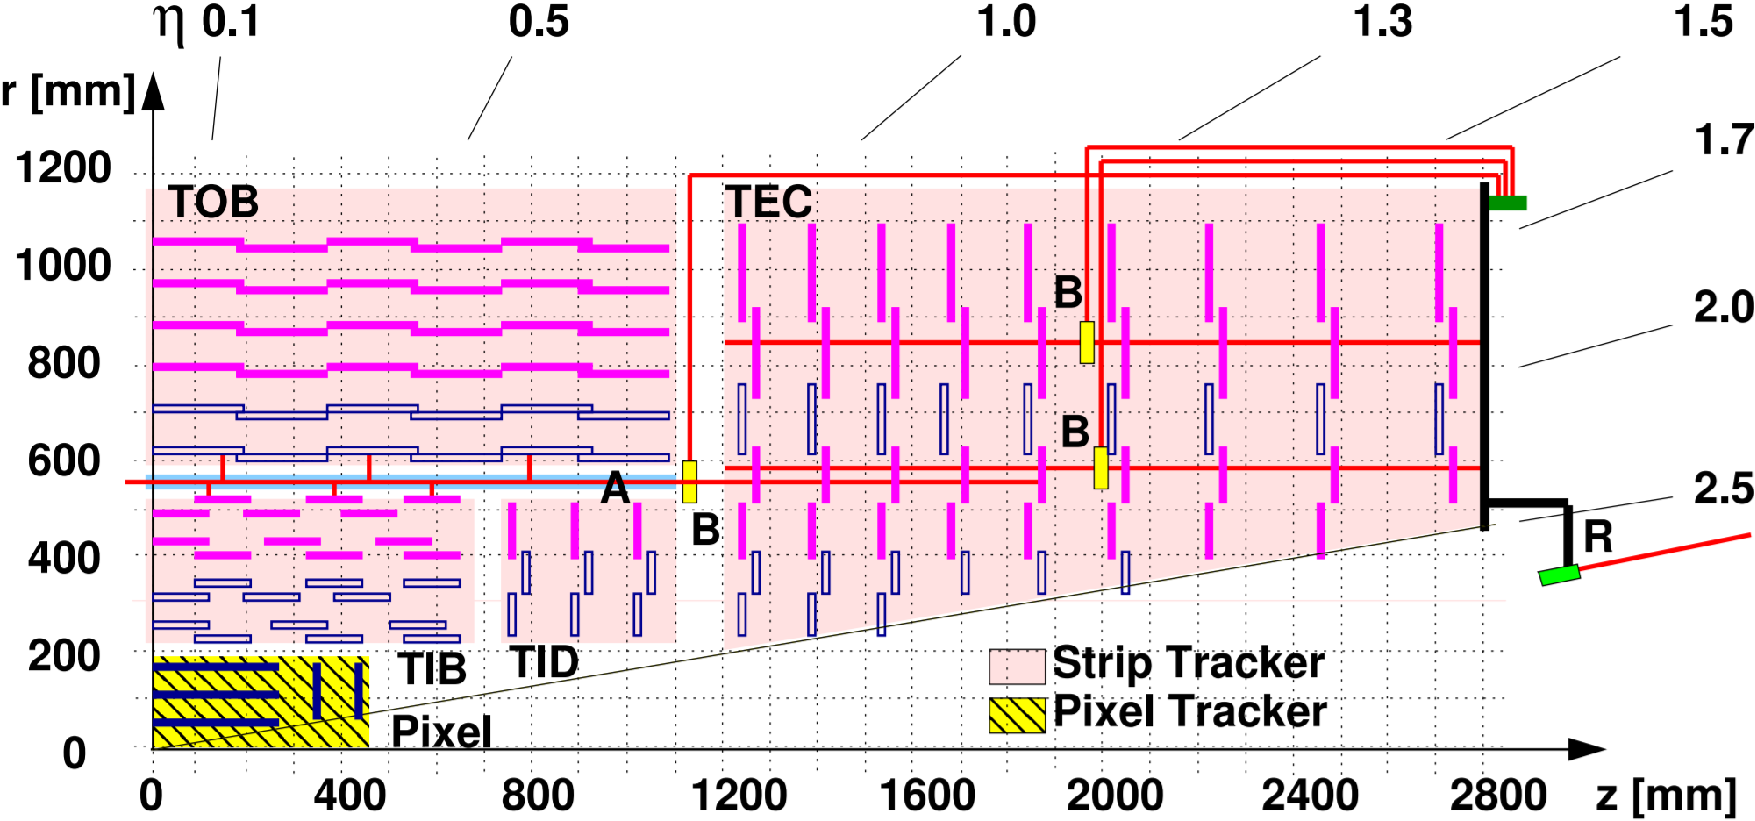
\includegraphics[width=0.85\textwidth]{fig/experiment/cms_siliconTracker.pdf}
  \caption{
    Layout of the CMS silicon strip tracker as seen in the $r$-$z$ plane.
    The Tracker Inner Barrel (TIB) has four inner barrel layers of silicon strips, which is closed off by the Tracker Inner Disks (TID) containing three disks in both of the endcaps.
    The Tracker Outer Barrel (TOB) has two double-sided layers of silicon strips outside of the TIB and is closed off by the Tracker EndCaps (TEC).
  }
  \label{fig:CMSsilicon}
\end{figure}

\subsection{Calorimeters}
\label{subsec:calorimeter}

% The calorimeters
The CMS detector is equipped with various calorimeters that are designed to measure the energies of particles emerging from the collision events.
Unlike the inner tracking system, the calorimeters are designed to abruptly halt any particles passing through them and record the energies of the stopped particles.
The electromagnetic calorimeter (ECAL) and preshower detector lie just outside of the silicon tracker and are designed to detect photons and electrons.
These are both encased by the hadron calorimeter (HCAL), which is used to measure hadron jets and neutrinos or exotic particles that result in missing transverse energy (MET\footnotemark).
\footnotetext{Transverse energy is typically written as \Et, which is why missing \Et is abbreviated as MET rather than MTE.}
Both the ECAL and HCAL are supplemented by the forward calorimeter, which is a Cerenkov-based detector that has electromagnetic and hadronic sections. % Check wording

\subsubsection{Electromagnetic Calorimeter}

% The ECAL
The ECAL consists of 61,200 lead tungstate (PbWO$_4$) crystal scintillators in the barrel region covering the pesudorapidity range $|\eta|<1.479$, with an additional 7,324 crystals in each of the two endcaps to close off the calorimeter.
Figure~\ref{fig:CMSECAL} shows an illustration of a module of the ECAL in the barrel region~\cite{Sakuma_2014}.
Scintillators are materials that emit light after absorbing ionizing radiation, which are attached to a photodetector and generate a current via the photoelectric effect.
These crystals were selected due to their density ($8.28\unit{g/cm^3}$), radiation length ($0.89\unit{cm}$), and Moli\`{e}re radius ($2.2\unit{cm}$), all of which allow for high resolution measurement of electron and photon energies while withstanding the harsh radiation levels of the LHC.
The photodetectors attached to the scintillators are also specially designed to operate in the $4\unit{T}$ magnetic field generated by the solenoid.
Additionally, around 80\% of the light from the scintillation effect is emitted in the LHC bunch crossing time of $25\unit{ns}$, which is adequate for detection purposes.
The crystals measure $22\times22\unit{mm^2}$ at the front face and $26\times26\unit{mm^2}$ at the rear face, corresponding to $0.0174\times0.0174$ in the $\eta$-$\phi$ plane, and have a length of $230\unit{mm}$.

\begin{figure}[htbp]
  \centering
  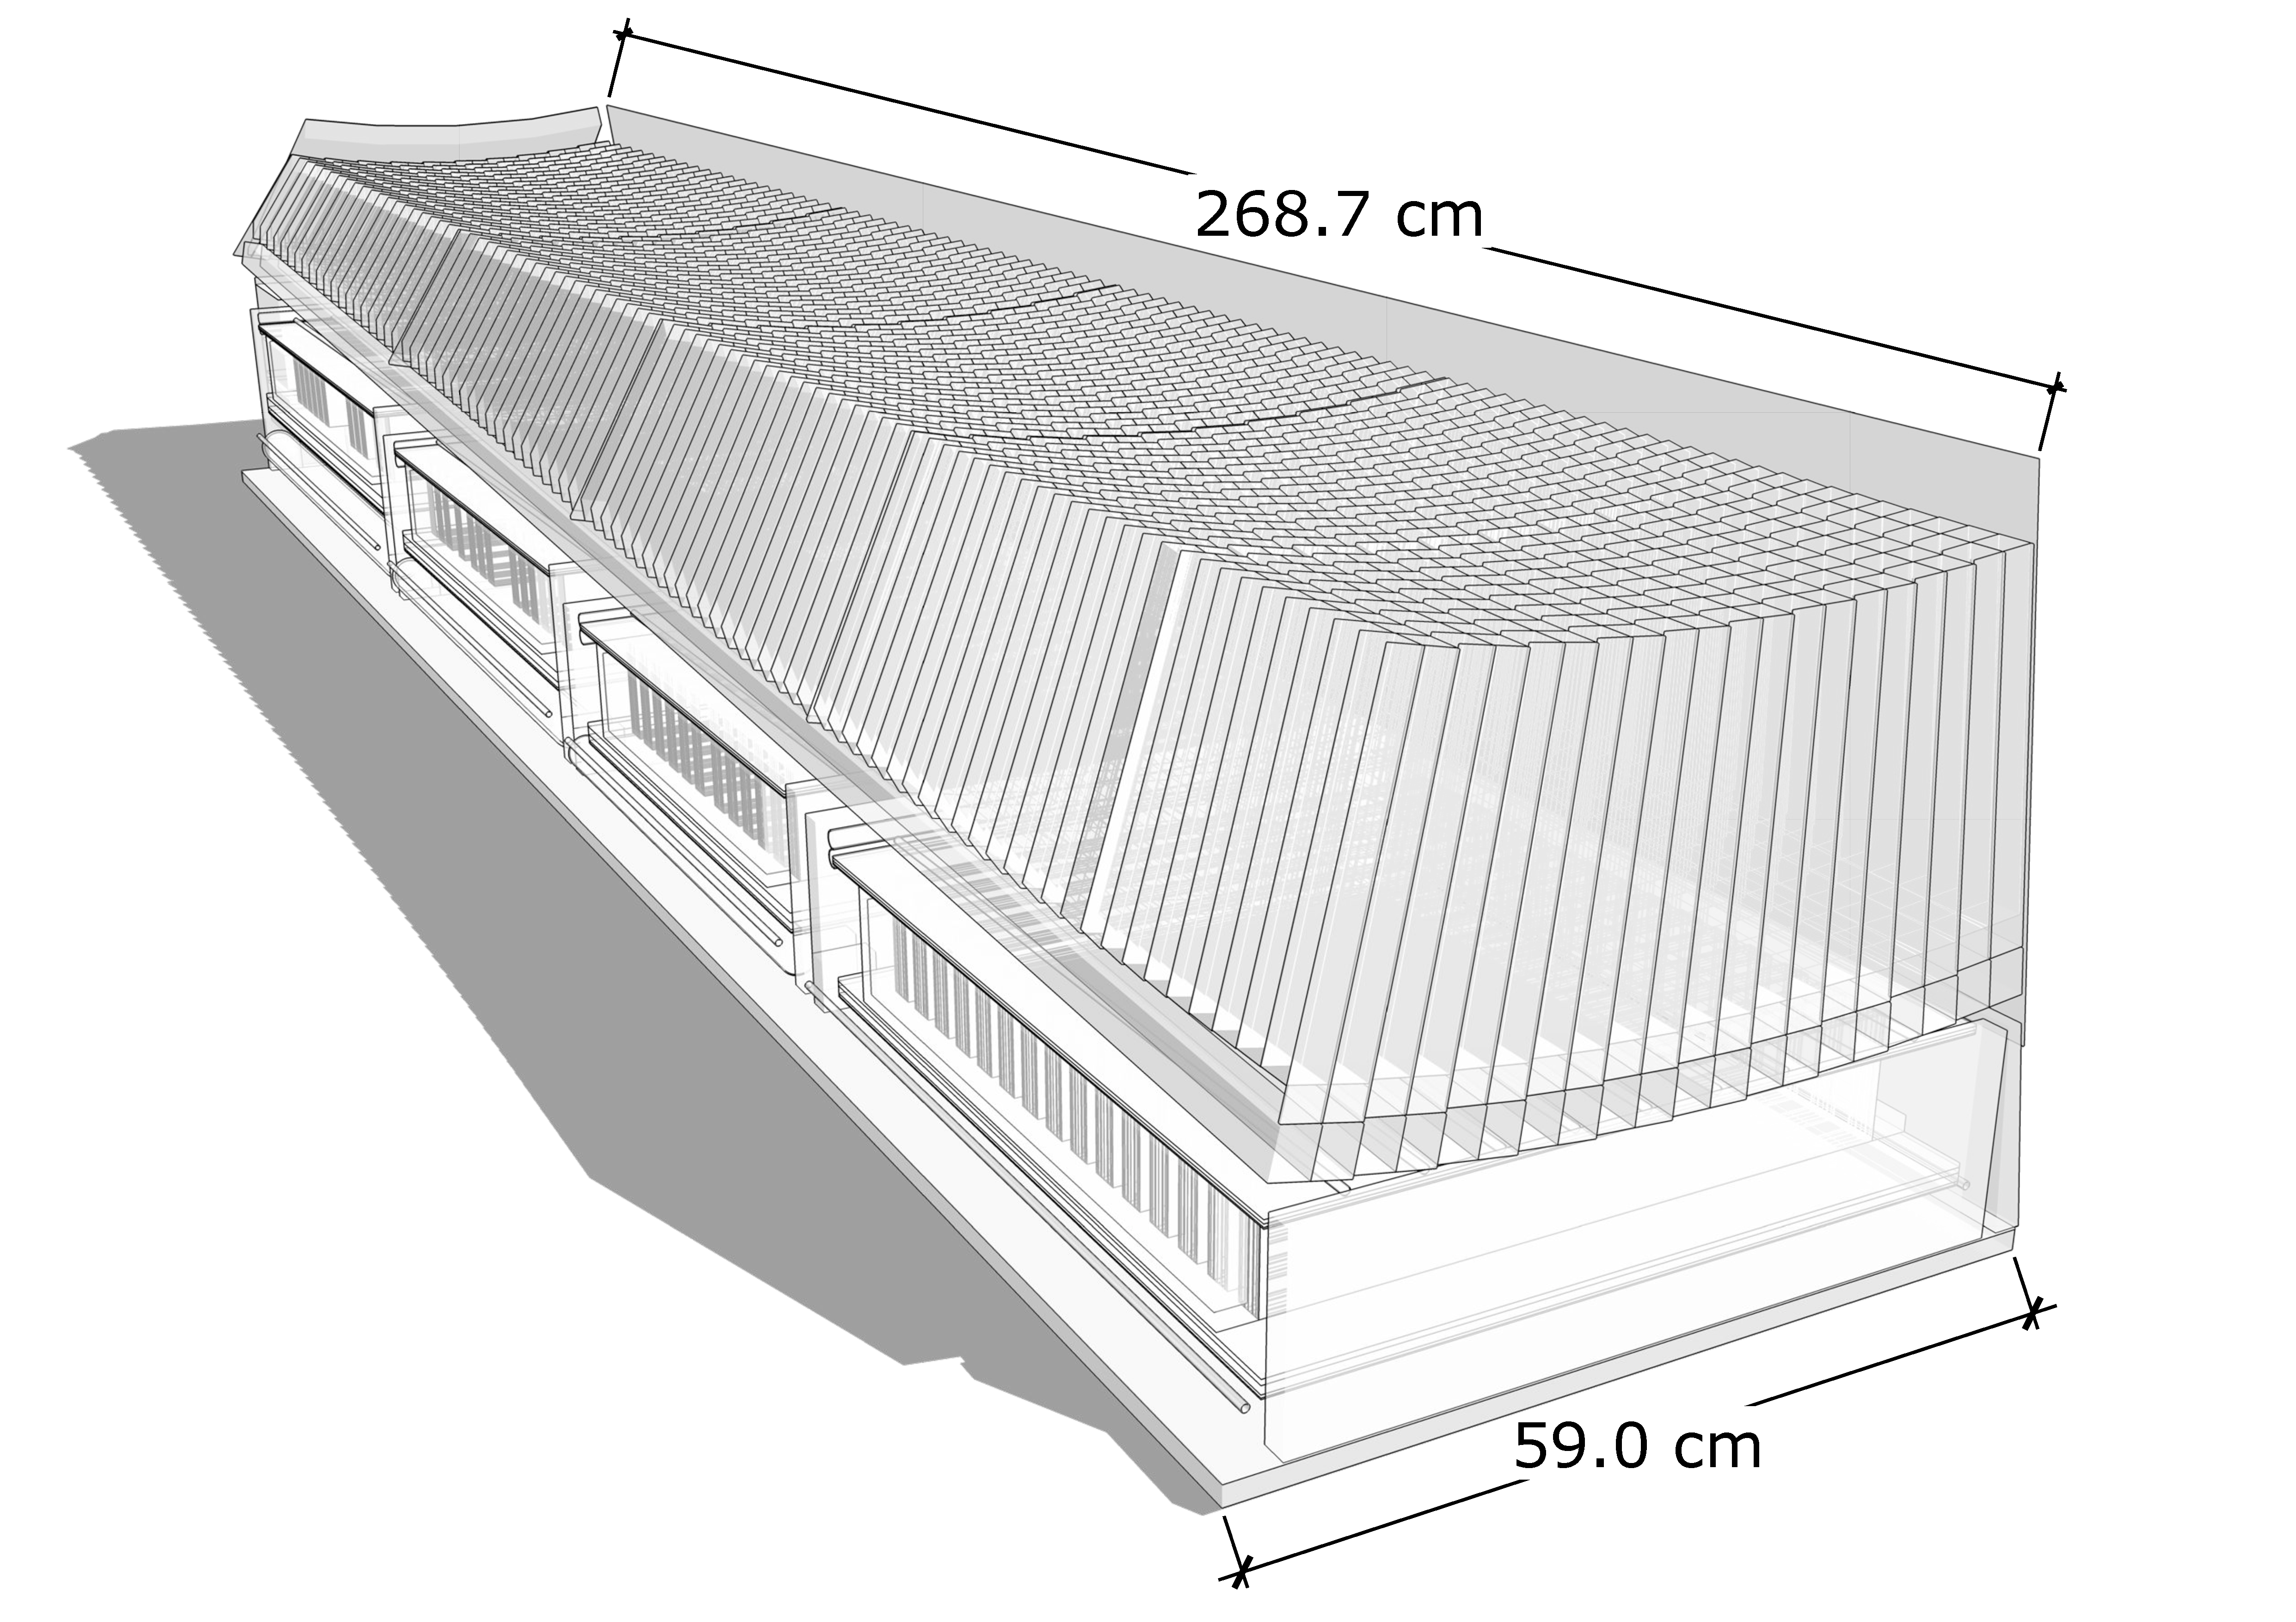
\includegraphics[width=0.65\textwidth]{fig/experiment/20130816_01_EB_module_1.pdf}
  \caption{
    Illustration of a module of the CMS ECAL in the barrel showing the layout of the lead tungstate scintillators.
    The scintillators emit light after absorbing ionizing radiation, each of which are attached to photodetectors and generate a current from the scintillation light.
  }
  \label{fig:CMSECAL}
\end{figure}

% Preshower detector
The ECAL also encloses a preshower detector that is designed to screen out neutral pions, as they can decay into two closely-spaced high-energy photons.
It also helps with identifying electrons against minimum ionizing particles and improves the position resolution for electrons and photons.
The preshower operates in the region $1.653<|\eta|<2.6$, and is closed off by two endcaps.
It is made of two layers, with lead radiators that generate electromagnetic showers when penetrated by incoming photons and electrons, and silicon strip sensors placed after each radiator to measure the deposited energies from the showers.
The detector strips are much finer than that of the ECAL crystals and are $2\unit{mm}$ wide, which allows for distinguishing individual photons from pion decays.

\subsubsection{Hadron Calorimeter}

% The hadron calorimeter
Outside of the ECAL lies the various layers of the HCAL, which is divided into four sections.
Figure~\ref{fig:CMSHCAL} shows the layout of the HCAL~\cite{Collaboration_2010_HCAL}.
The first of these is the barrel (HB), which covers the pseudorapidity range $|\eta|<1.3$.
The HB has 36 azimuthal wedges that are constructed out of brass absorber plates bolted together in a staggered geometry.
Between the layers of brass are tiles of plastic scintillators that cover an area of $0.087\times0.087$ in the $\eta$-$\phi$ plane.
To maximize the coverage of the HCAL and obtain an accurate reading of the deposited energies, the wedges are bolted together so as to allow for no more of a gap than $2\unit{mm}$ between the wedges.
The endcaps (HE) cover the HB section and extend over the pseudorapidity range $1.3<|\eta|<3$.
Scintillators in this region have a granularity of $\Delta\eta\times\Delta\phi=0.087\times0.087$ in the region $|\eta|<1.6$ and $\Delta\eta\times\Delta\phi\approx0.017\times0.017$ for $|\eta|\geq1.6$.
The outer calorimeter (HO) sits just outside of the vacuum tank of the solenoid, divided into five rings aligned along the axis of the LHC beam.
The central ring of the HO has two layers of scintillators at radii of $3.82\unit{m}$ and $4.07\unit{m}$, while the other rings only have a single scintillator layer at $4.07\unit{m}$.
Finally, the forward calorimeter (HF) consists of two detectors that are $11.2\unit{m}$ away from the interaction point on both sides of CMS.
The HF faces the unique challenge of dealing with intense radiation, as most of the energy from the collisions is directed into the forward regions of the detector.
For this reason, quartz fibers were used as the scintillation material and the signal is generated by Cherenkov radiation from charged particles passing through the medium.

\begin{figure}[htbp]
  \centering
  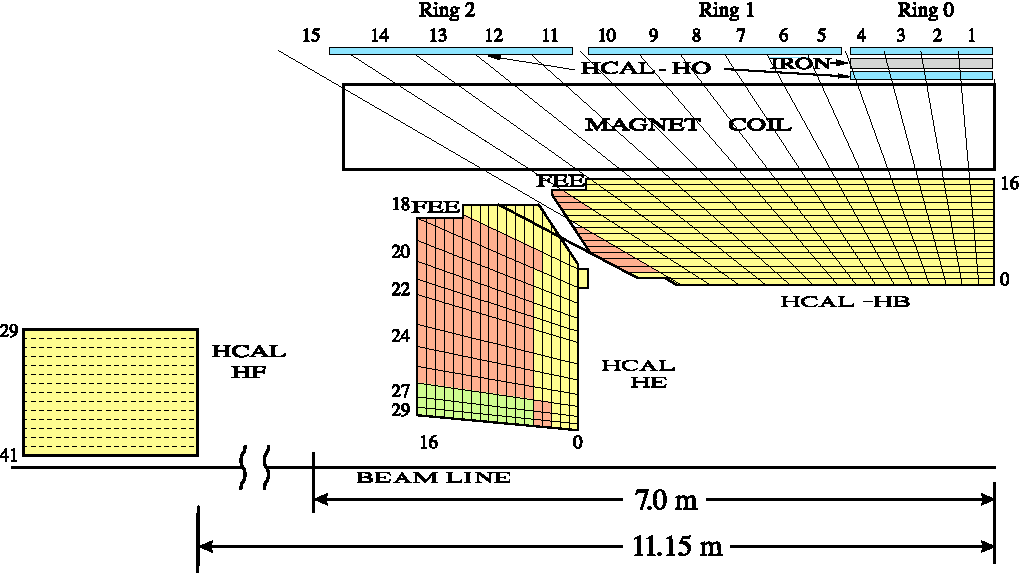
\includegraphics[width=0.75\textwidth]{fig/experiment/HCAL-HB-HE-HO-HF.pdf}
  \caption{
    Layout of the HCAL in the $r$-$z$ plane.
    The HCAL surrounds the ECAL and has four sections denoted by the barrel (HB), endcaps (HE), outer calorimeter (HO), and forward calorimeter (HF).
    The scintillation material in the HB, HE, and HO sections is made of plastic, while the HF section uses quarts fibers in order to withstand the intense radiation in the forward region of the detector.
  }
  \label{fig:CMSHCAL}
\end{figure}

\subsection{Muon Tracking System}
\label{subsec:muonTrack}

% The muon system
The muon system is of central importance to the CMS detector.
From its inception as a detector, it was recognized that muons would be one of the primary tools for reconstructing collision events.
One reason for this is the fact that final states with muons present offer some of the best results for mass resolution, thereby increasing the discovery potential for new physics.
This was one of the considerations taken into account when designing the CMS detector to optimize for the observation of the Higgs before it was discovered.
The so-called $H\to ZZ^{(*)}\to 4\ell$ ``golden channel'' has the cleanest signal when all four of the leptons in the final state are muons~\cite{Gainer_2011}.
Moreover, muons are expected to be produced in many decay events for exotic particle from BSM theories.
As such, the muon system is designed to provide robust and accurate muon identification, momentum measurement, and triggering for events.
This is achieved thanks to the combination of the strong solenoidal magnetic field and the flux return yoke.
The return yoke allows for pulling the magnetic field lines from the solenoid to the outer region where the muon detection chambers are located, and it also screens out hadrons by absorbing them.
The detection hits in the layers of the muon chambers then allow for reconstructing the charge and momentum of the muons.

% Detection chambers
There are three kinds of gaseous detection chambers that are used to identify and measure muons: drift tubes (DTs), cathode strip chambers (CSCs), and resistive plate chambers (RPCs).
The outer region of CMS has 250 DTs in the barrel region covering pseudorapidities of $|\eta|<1.2$, while the endcaps on both ends of CMS have 540 CSCs covering the region $0.9<|\eta|<2.4$.
The RPCs are distributed throughout both regions of CMS, with 480 in the barrel and 576 in the endcaps.
In total, there are 1846 muon chambers present on the detector, with the chambers distributed among four layers in both the barrel and endcap regions to allow for track reconstruction. % Check numbers
The barrel region is split up into five concentric wheels that are numbered from $-2$ to $+2$, with wheel 0 centered at the interaction point.
Figure~\ref{fig:CMScrosssec} shows a cross section of the CMS detector in the $r$-$z$ plane as configured during Run 2, with DTs, CSCs, and RPCs labeled~\cite{Sirunyan_2018_CMS}.

\begin{figure}[htbp]
  \centering
  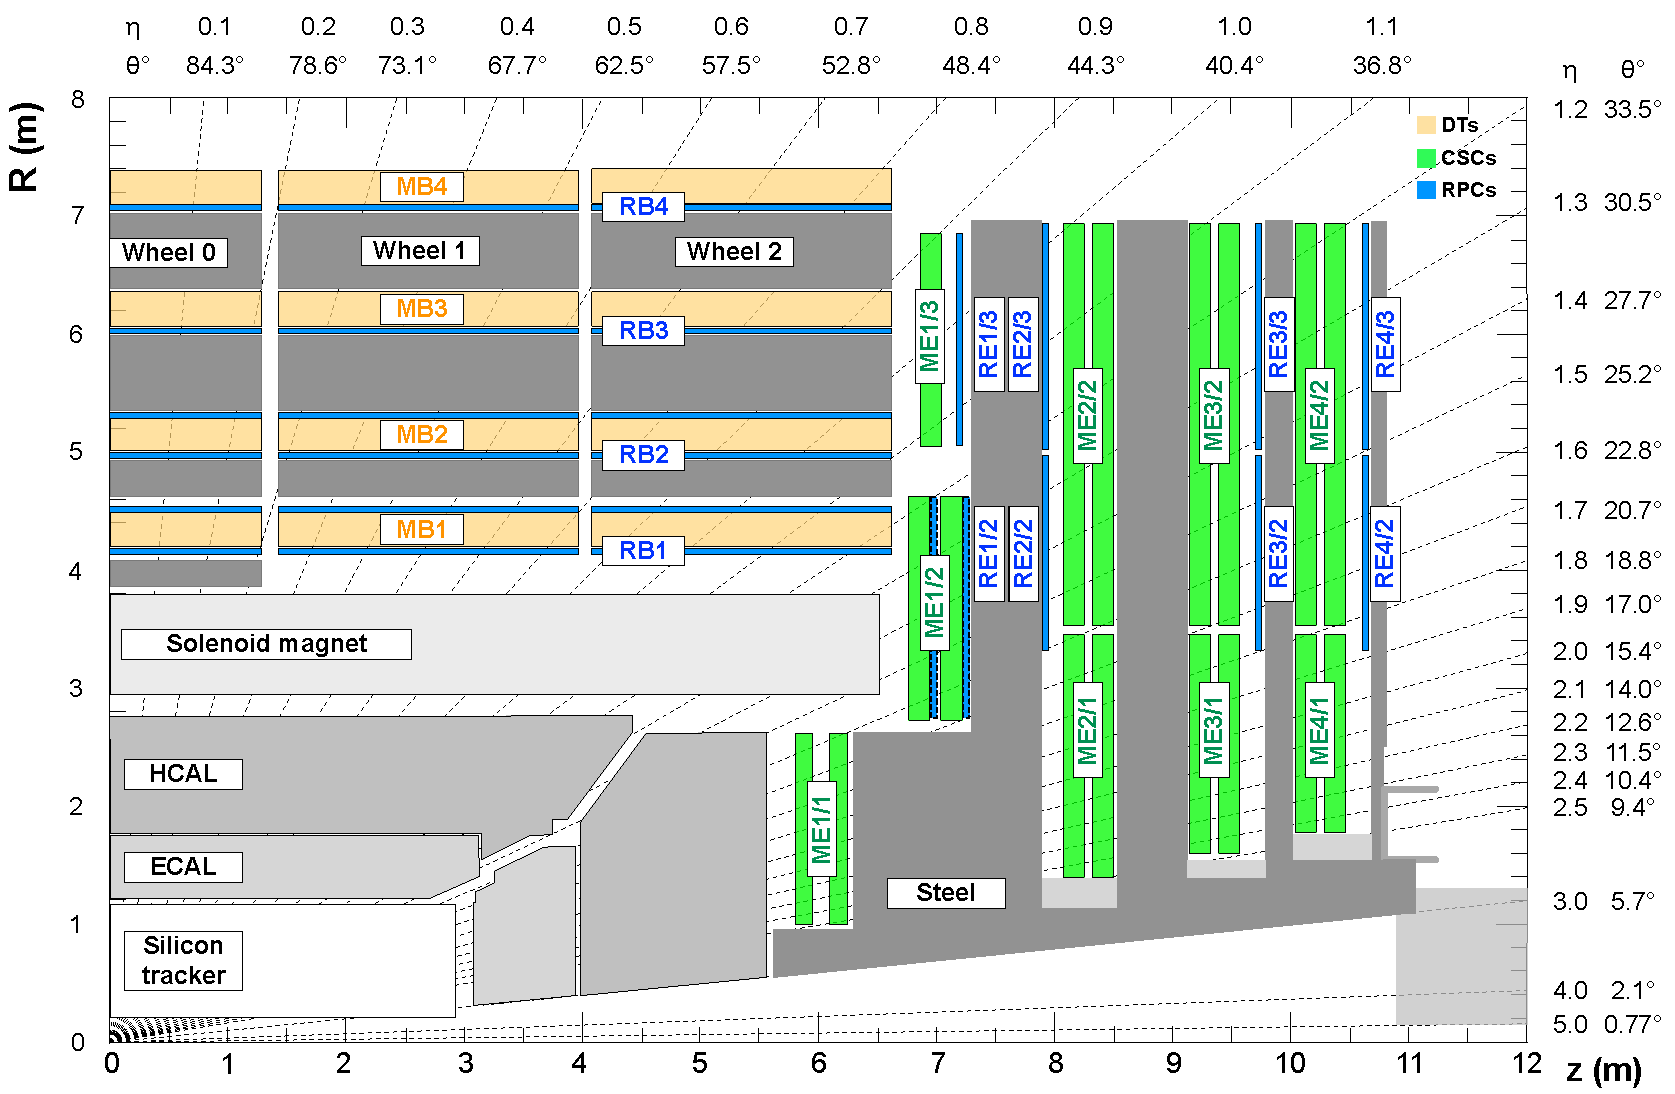
\includegraphics[width=0.85\textwidth]{fig/experiment/cms_crosssec.pdf}
  \caption{
    cross section of the CMS detector in the $r$-$z$ plane as configured during Run 2.
    The barrel region contains a combination of drift tubes and resistive plate chambers distributed among five concentric wheels surrounding the detector, covering a pseudorapidity range of $|\eta|<1.2$.
    The endcaps on either side cover the range $0.9<|\eta|<2.4$, and have combinations of cathode strip chambers and resistive plate chambers present.
    There are 250 drift tubes and 480 resistive plate chambers in the barrel, and 540 cathode strip chambers and 576 resistive plate chambers in the endcaps, making a total of 1846 muon chambers distributed throughout CMS.
    Both the barrel and endcaps have four layers of muon chambers to allow for track reconstruction.
  }
  \label{fig:CMScrosssec}
\end{figure}

\subsubsection{Drift Tubes}

% The DT system
The DT system in the barrel region is distributed among the four layers present in each wheel surrounding the interaction point, with the layers referred to as stations.
The stations are numbered according to how close they are to the interaction point, with station 1 being the innermost layer and station 4 being the outermost.
Each drift tube contains a gaseous mix of Ar (85\%) and CO$_2$ (15\%), with sensitive wires inside of the tubes held at a specified potential.
An illustration of an individual drift tube cell can be seen in figure~\ref{fig:CMSDTcell}~\cite{Abbiendi_2019}.
As muons pass through the gas, they impart enough ionization energy to knock off electrons from the atoms of the gas, which are then attracted to the wire and cause a cascade of additional electrons from the gas to be deposited onto the wire and cause a current.
The muon's position can then be inferred from where the electrons hit the wire, and how far the muon was from the wire.
Additionally, the muon track and momentum can be reconstructed by using multiple detection hits from different stations in the barrel.
Each DT allows for a position resolution of $0.25\unit{mm}$.

\begin{figure}[htbp]
  \centering
  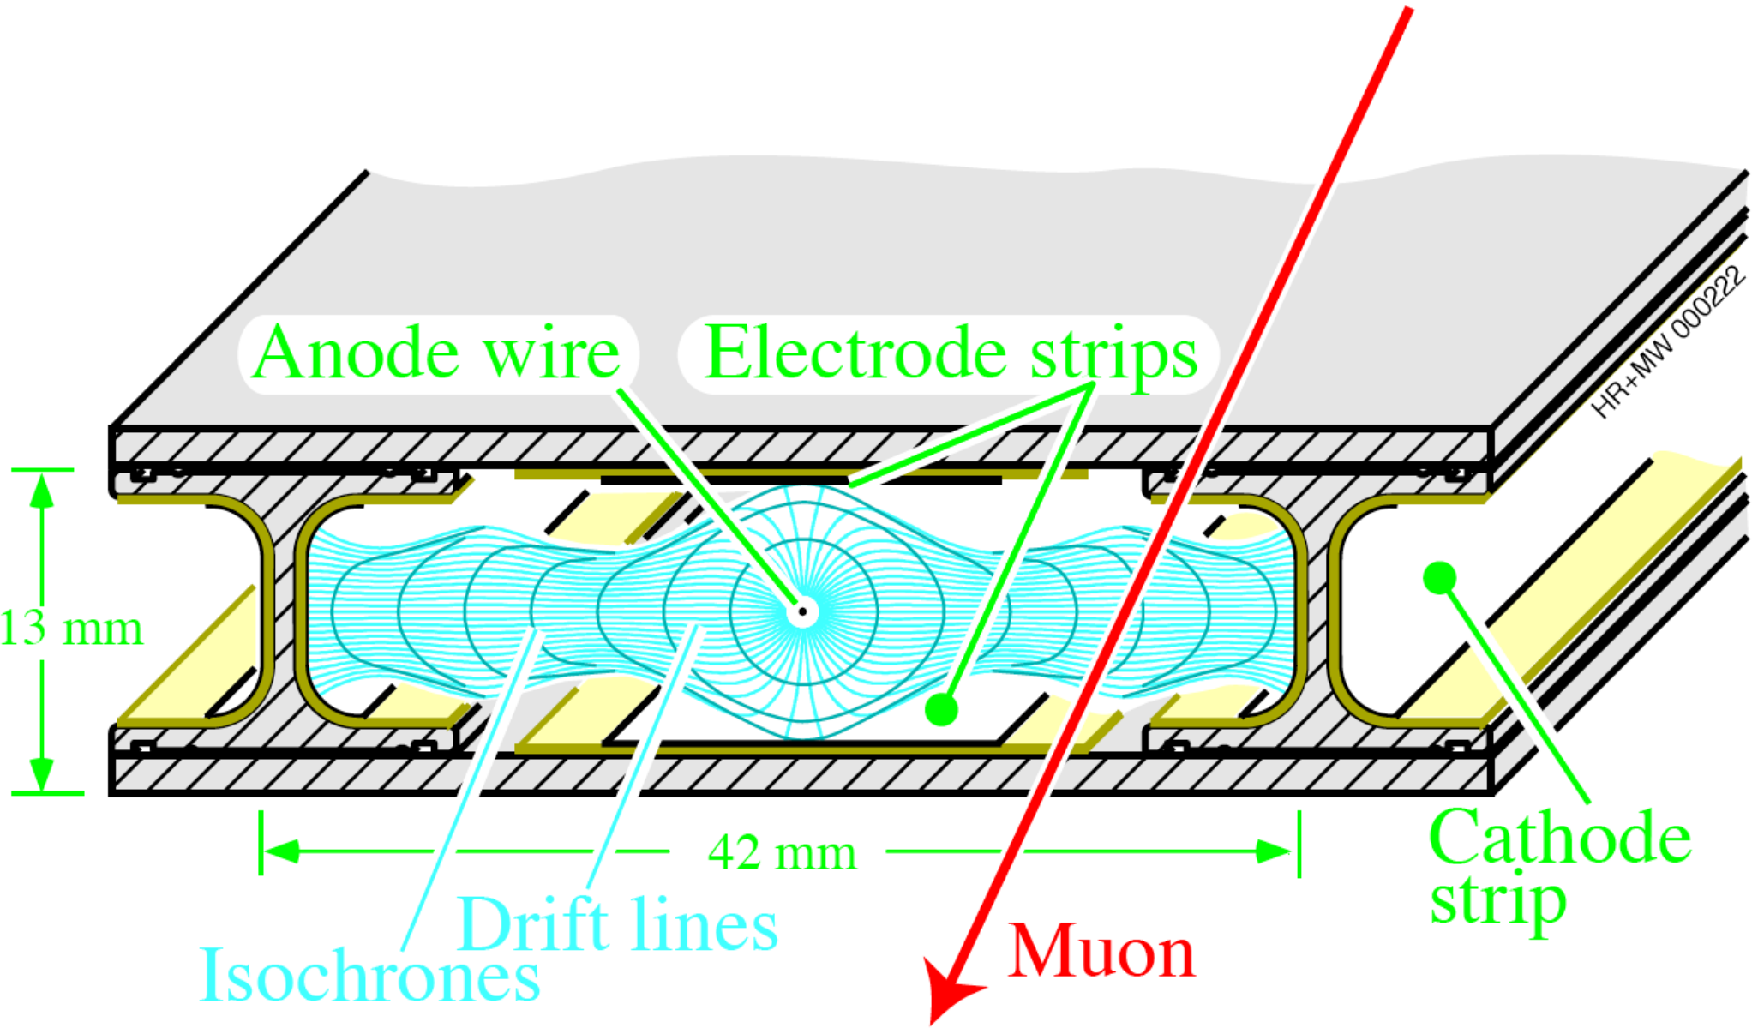
\includegraphics[width=0.65\textwidth]{fig/experiment/cms_DTcell.pdf}
  \caption{
    Illustration of a drift tube cell.
    As muons pass through the cell, they ionize the gas and cause a cascade of electrons that deposit onto the anode wire and generate a current.
    The current is readout by the detector and allows for measuring muon momentum.
  }
  \label{fig:CMSDTcell}
\end{figure}

\subsubsection{Cathode Strip Chambers}

% The CSC system
The CSCs in the endcaps operate under a similar principle to that of the DTs in the barrel region.
They are made of trapezoidal panels and have a gas mix of Ar (40\%), CO$_2$ (50\%), and CF$_4$ (10\%).
Figure~\ref{fig:CMSCSC} shows a cut-away diagram of a CSC chamber~\cite{collaboration_2013}.
Inside of the CSCs are arrays of positively-charged anode wires and negatively-charged cathode copper strips that are perpendicular to each other.
When muons ionize the gas after passing through the chamber, they cause an avalanche of electrons to deposit onto the wire and generate a current, but they also cause an induced charge on the copper strips.
This allows for a precise measurement of $\phi$ for the passing muons and a coarse measurement of $r$ from the anode wires, resulting in a $0.2\unit{mm}$ resolution position measurement, as well as a fast time measurement.

\begin{figure}[htbp]
  \centering
  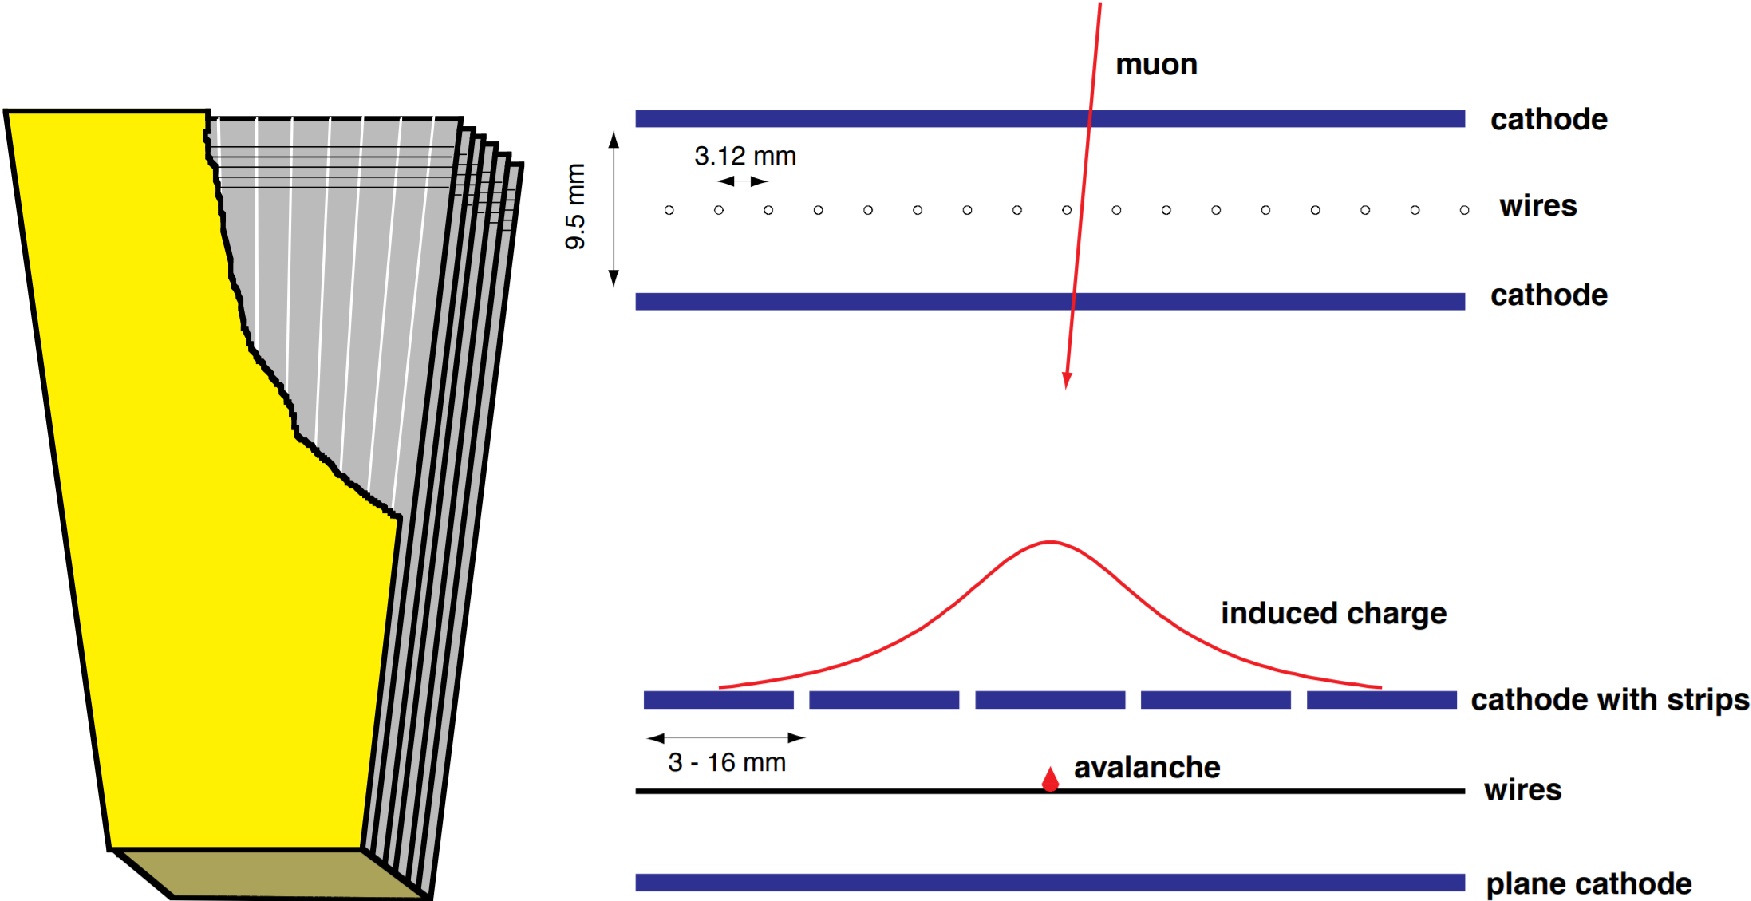
\includegraphics[width=0.75\textwidth]{fig/experiment/cms_csc.pdf}
  \caption{
    Cut-away diagram of a CSC (left) with an illustration of the ionization mechanism (right).
    As muons ionize the gas, the resulting electron avalanche deposits onto the wires and generate a current, while also inducing a charge onto the cathode strips.
    This gives a measurement of the muon position for both $\phi$ and $r$.
  }
  \label{fig:CMSCSC}
\end{figure}

\subsubsection{Resistive Plate Chambers}

% RPCs
RPCs are used to supplement the DTs in the barrel and the CSCs in the endcaps.
They are gaseous detectors that consist of two parallel plastic plates with high resistivity, one being a positively-charged anode and the other a negatively-charged cathode.
Figure~\ref{fig:CMSRPC} shows an example of a double gap RPC design~\cite{kumari2020improvedrpc}.
The gaseous mix in the RPCs is C$_2$H$_2$F$_4$ (95.2\%), isoC$_4$H$_{10}$ (4.5\%), and SF$_6$ (0.3\%).
The electron cascade caused by the ionization of a passing muon generates a signal on external detecting strips, which allows for a coarse spatial measurement, but a very fast time measurement ($1\unit{ns}$) that is shorter than the $25\unit{ns}$ between each bunch crossing.
Their fast response time is used in the trigger system in order to determine whether or not event data should be saved based on the measured muon momentum.

\begin{figure}[htbp]
  \centering
  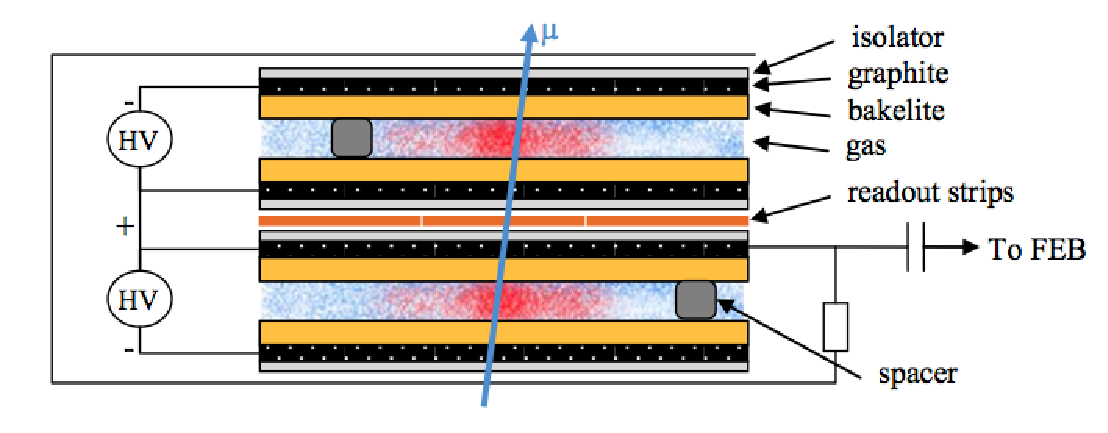
\includegraphics[width=0.65\textwidth]{fig/experiment/rpc_schema.pdf}
  \caption{
    Illustration of a double gap RPC design.
    The electron cascade generated by the ionization process induces a signal on the readout strips, which gives a coarse spatial measurement.
    DTs and CSCs are supplemented by RPCs that are used by the trigger system due to their fast response time.
  }
  \label{fig:CMSRPC}
\end{figure}

\subsection{Trigger System}
\label{subsec:trigger}

% Motivation for the trigger system
One of the unique challenges facing detectors at the LHC is the large amount of collision events that occur at the interaction points.
Proton-proton collisions occur every $25\unit{ns}$, corresponding to a rate of $40\unit{MHz}$.
With 20 simultaneous $pp$ collisions for every bunch crossing, this corresponds to $8\times10^8$ interactions every second.
It is not possible to meet the hardware demands for recording every single collision event, nor would it be prudent to do so since most events are soft collisions between protons that do not reveal any new physics.
Thus, the trigger system is needed in order to select for high-energy events of interest, while also recording them at a reasonable rate that allows for long-term storage.

% Trigger system overview
The trigger system has two levels, consisting of a Level-1 (L1) Trigger, and a High-Level Trigger (HLT).
The L1 Trigger is hardware-based and is comprised of custom-designed electronics that uses data from the calorimeters and muon system.
The HLT is software-based and consists of a conventional CPU farm, which has access to a complete readout from the L1 Trigger and is able to perform more advanced calculations with the data.
The trigger system as whole reduces the rate by a factor of $10^6$, with the L1 Trigger designed to have an output rate of 100 kHz.
In practice, the L1 Trigger is not operated at its maximum output and instead runs at 30 kHz as a safety measure.

\subsubsection{Level-1 Trigger}

% Level 1 trigger
The architecture of the L1 trigger can be seen in figure~\ref{fig:L1Trigger}~\cite{cmscollaboration2020performance}.
At the local level, the L1 Trigger consists of Trigger Primitive Generators (TPG) that are activated by track segments or hit patterns in muon chambers, and energy deposits in the calorimeters.
The trigger primitives are then used by the Regional Triggers to form trigger objects for candidate particles, such as electrons, photons, and muons.
These objects have to be ranked and sorted based on their energy, momenta, and quality.
The highest rank objects are then transferred to the Global Trigger and are evaluated to determine whether or not they will be passed onto the HLT.
This is determined by the Trigger Control System (TCS), which will then pass a Level-1 Accept (L1A) decision back to the Global Trigger.
The allowed latency between the a single bunch crossing and the L1A decision in the L1 Trigger is $3.2\unit{\micro s}$, which requires the entire process to be pipelined so that the L1 Trigger may operate continuously.

\begin{figure}[htbp]
  \centering
  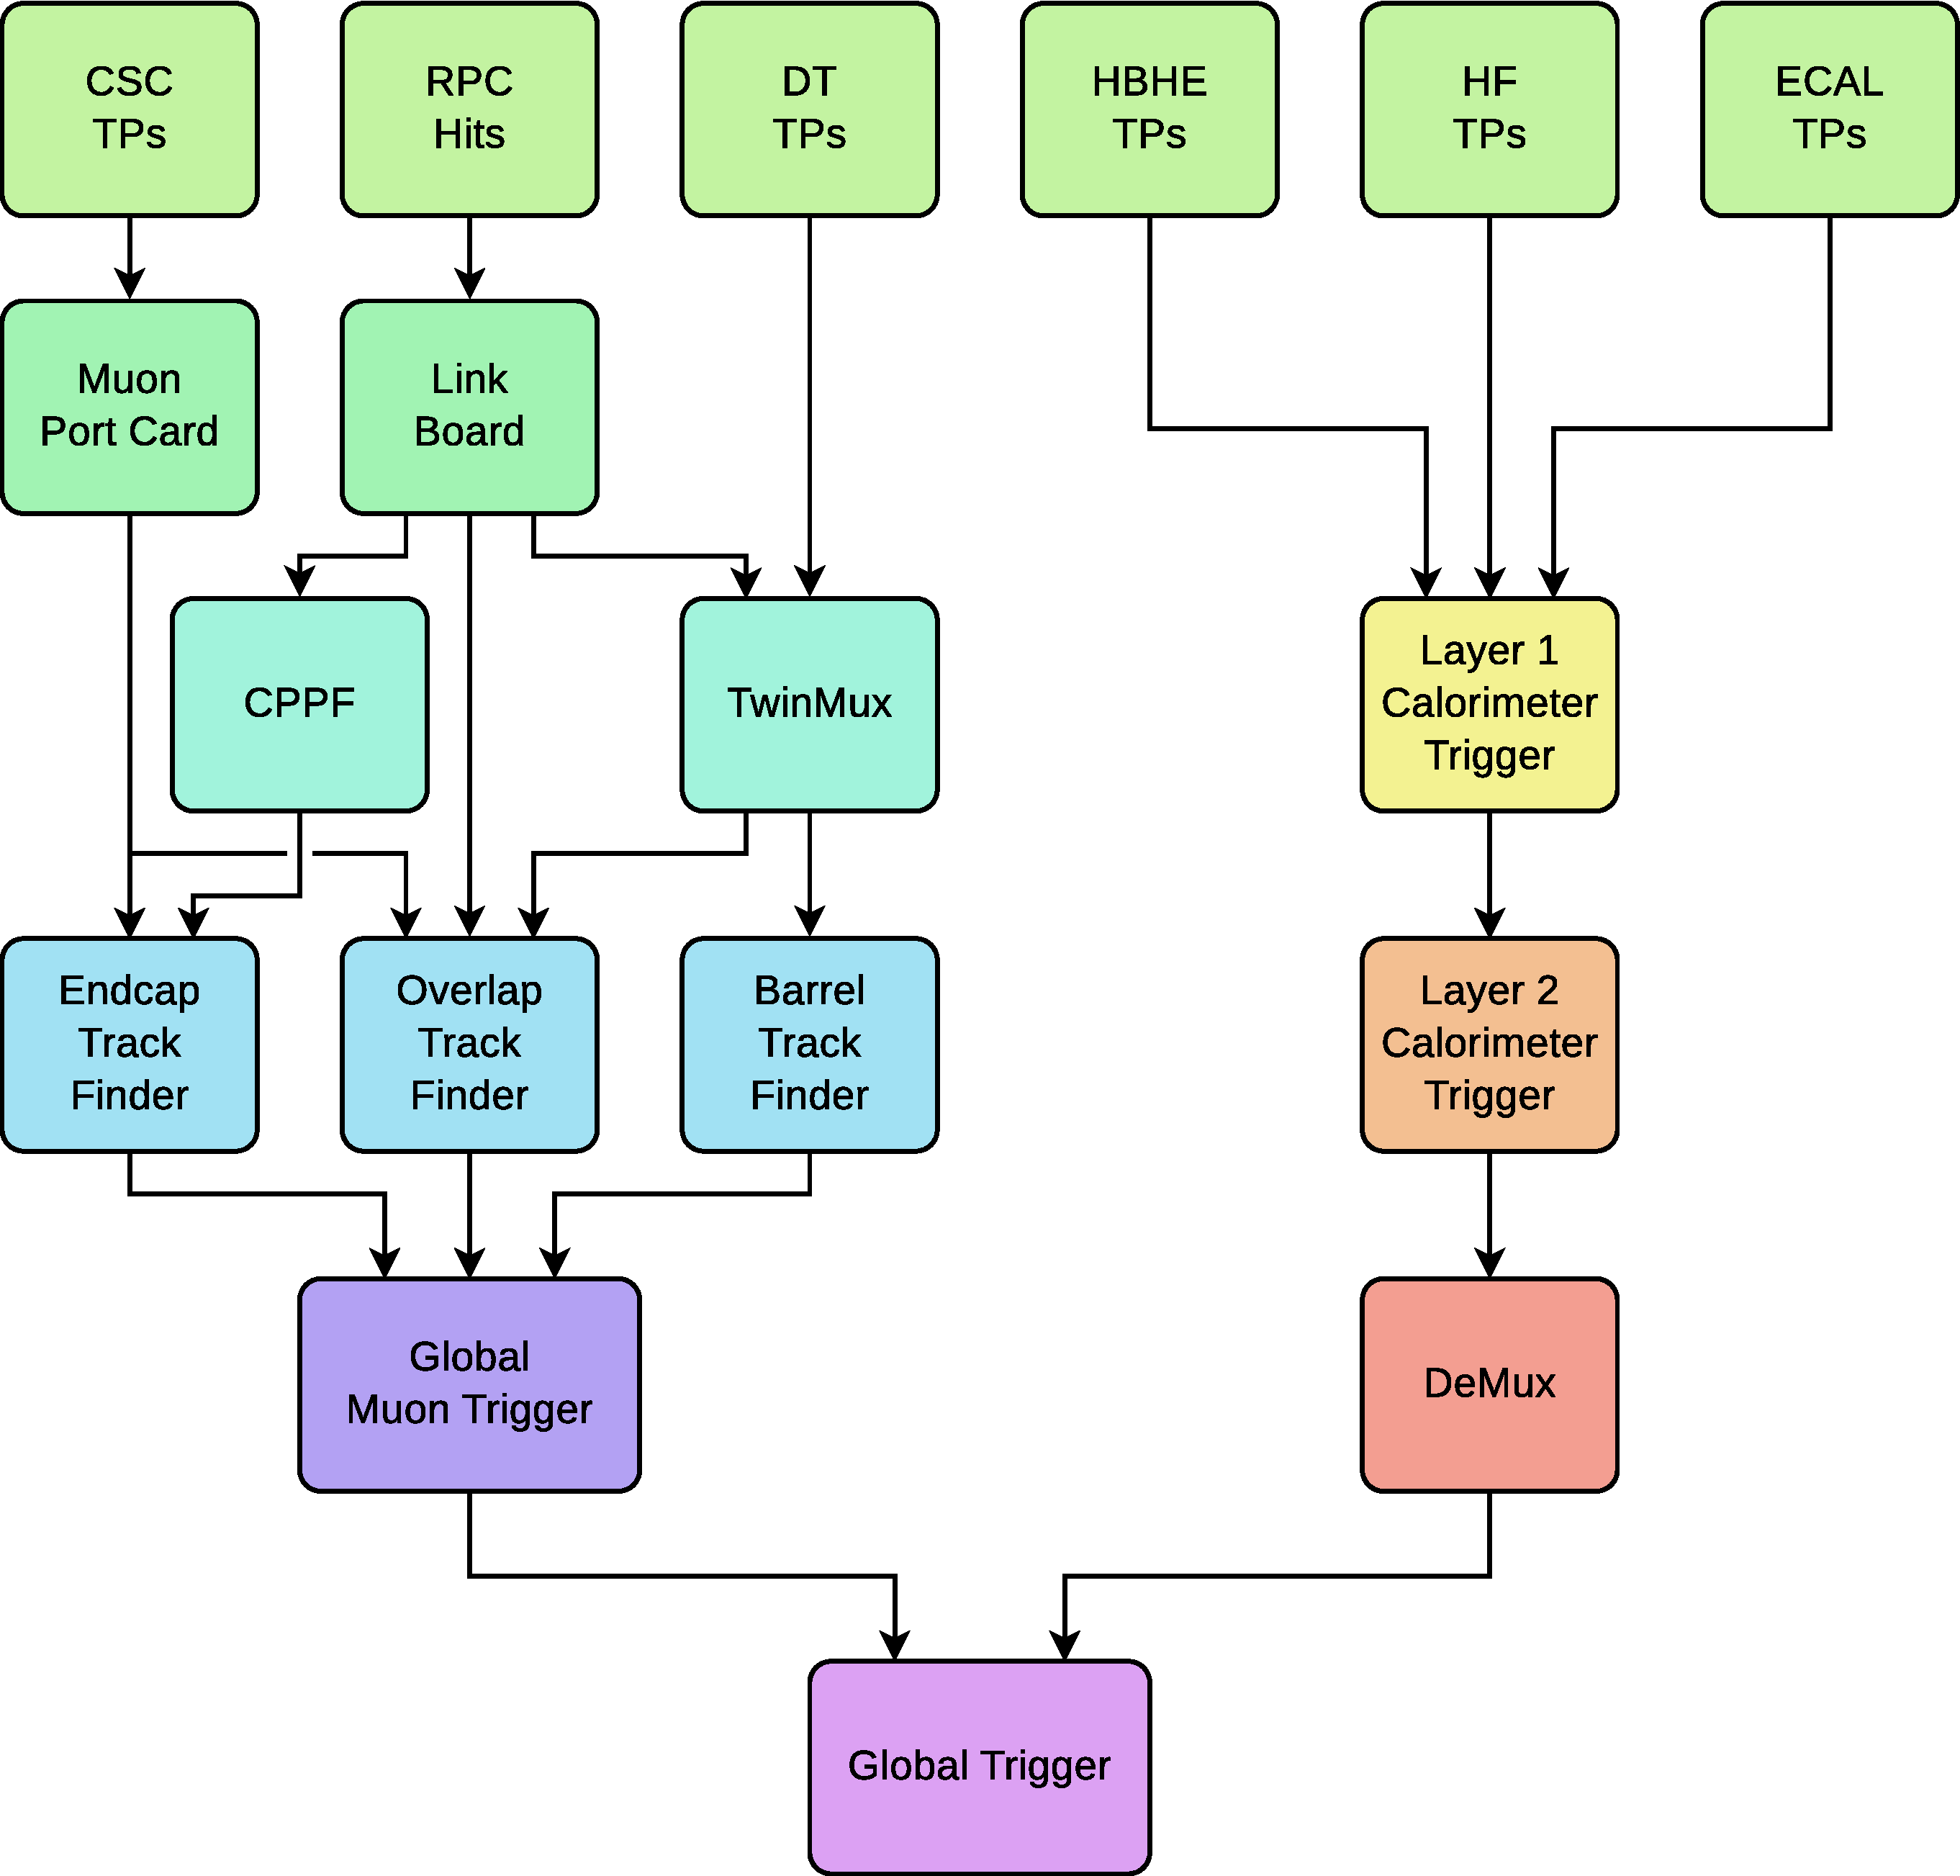
\includegraphics[width=0.65\textwidth]{fig/experiment/cms_L1trigger.pdf}
  \caption{
    Illustration of the L1 Trigger architecture as configured during Run 2.
    The Trigger Primitives (TPs) are generated by track segments or hit patterns in muon chambers, and energy deposits in calorimeters.
    These objects are ranked and sorted by energy, momenta, and quality, which are then passed onto the Global Trigger to determine whether or not the events will be kept and passed to the HLT.
  }
  \label{fig:L1Trigger}
\end{figure}

\subsubsection{High Level Trigger}

% High level trigger
After receiving the L1A signal, the complete readout data from the rest of the detector is sent to the HLT to be further analyzed.
The HLT uses various algorithms to reconstruct the full event and performs tasks such as matching tracks from the inner tracker to muon detection hits in the chambers, or identifying high-energy photons.
Since the HLT is software-based, the algorithms used to reconstruct the events have changed over the operational history of the CMS detector~\cite{Trocino_2014}.
After passing through the HLT, the events are then recorded for offline analysis, and the rate of recorded events after passing through the trigger system as a whole is cut down to be on the order of only a few $10^2\unit{Hz}$.
The recorded events are then passed onto the Data Acquisition (DAQ) system~\cite{Cittolin:578006}.
